\documentclass[aspectratio=169, 9pt,t]{beamer}
\graphicspath{{figures/}} % Setting the graphicspath

% Theme settings
\usetheme{Madrid}
\usecolortheme{default}
\setbeamertemplate{navigation symbols}{}   % removes navigation symbols such as 'next page'
\setbeamertemplate{footline}{}             % remove line with name, date, page nr.
\setbeamercolor*{frametitle}{bg=white}     % remove background from frametitle
\usepackage{caption}
% \captionsetup[figure]{labelformat=empty}% redefines the caption setup of the figures environment in the beamer class.
\setbeamersize{text margin left=20pt,text margin right=10pt}
\usefonttheme[onlymath]{serif} % makes beamer math look like article math
\usepackage{hyperref}

%======================= title page info =======================
\title{Recent progress in global PDF determination and the path to N$^3$LO}
\subtitle{Based on 2401.08749, 2401.10319, and 2402.18635 }
\date{Joint Northern UK Journal Club  \\[0.1cm] 23 April 2024}
\author{Roy Stegeman}
\institute{\small The University of Edinburgh}


%======================= page numbering =======================
\addtobeamertemplate{navigation symbols}{}{ \usebeamerfont{footline}
  \insertframenumber / \inserttotalframenumber \hspace*{2mm} \\ \vspace*{1mm}
}


%=================================== colors ====================================
\definecolor{RoyBlue}{RGB}{22, 46, 69}
\definecolor{RoyGrey}{RGB}{64, 88, 128}

\newcommand{\hlme}[1]{{\color{red}\bf #1}} % highlight me

\setbeamercolor{structure}{fg=RoyBlue} % itemize, enumerate, etc
\setbeamercolor{frametitle}{fg=RoyGrey}
\setbeamercolor{section in head/foot}{bg=RoyBlue}


%======================= add progress dots to headline =========================
% \setbeamertemplate{headline}{%
%     \begin{beamercolorbox}[ht=4mm,dp=4mm]{section in head/foot}
%         \insertnavigation{\paperwidth}
%     \end{beamercolorbox}%
% }%
% \makeatother


%======================= add section title page ================================
\AtBeginSection[]{
  \begin{frame}
  \vfill
  \centering
    \usebeamerfont{title}\insertsection\par%
  \vfill
  \end{frame}
}


%=================================== titlepage =================================
\titlegraphic{\vspace*{6mm}
  
\includegraphics[height=1.5cm]{logos/edi_logo.png} \hspace{10mm}
  % 
\includegraphics[height=0.8cm]{logos/nnpdf_logo_official.pdf} \hspace{10mm}
  
\includegraphics[height=1.5cm]{logos/higgs_logo.jpg}
}

\defbeamertemplate{title page}{noinstitute}[1][]
{
  \vbox{}
  \vfill
  \begingroup
    \centering
    \begin{beamercolorbox}[sep=8pt,center,#1]{title}
      \usebeamerfont{title}\inserttitle\par%
      \ifx\insertsubtitle\@empty%
      \else%
        \vskip0.25em%
        {\usebeamerfont{subtitle}\usebeamercolor[fg]{subtitle}\insertsubtitle\par}%
      \fi%
    \end{beamercolorbox}%
    \vskip2em\par
    \begin{beamercolorbox}[sep=0pt,center,#1]{author}
      \usebeamerfont{author}\insertauthor
    \end{beamercolorbox}
  \begin{beamercolorbox}[sep=0pt,center,#1]{author}
    \usebeamerfont{institute}\insertinstitute
  \end{beamercolorbox}
  \vspace*{8pt}
  \vspace*{16pt}
    \begin{beamercolorbox}[sep=0pt,center,#1]{date}
      \usebeamerfont{date}\insertdate
    \end{beamercolorbox}\vskip0.5em
    {\usebeamercolor[fg]{titlegraphic}\inserttitlegraphic\par}
  \endgroup
  \vfill
}

\makeatletter
\setbeamertemplate{title page}[noinstitute][colsep=-4bp,rounded=true,shadow=\beamer@themerounded@shadow]
\makeatother


\begin{document}
{
\setbeamertemplate{headline}{} % remove headline from titlepage
\begin{frame}
  \titlepage
\end{frame}
}

\setbeamertemplate{enumerate items}[default]

\pgfdeclarelayer{bg}    % declare background layer
\pgfsetlayers{bg,main}  % set the order of the layers (main is the standard layer)


% SLIDES =======================================================================
\newcommand{\nn}{\vspace*{1em}}

\section*{PDF determination in NNPDF}

\begin{frame}{Introduce NNPDF}
\end{frame}



\section*{Motivation}

\begin{frame}{Motivation}
  $\sigma(x,Q^2)=\sum_i \int_x^1 \frac{dz}{z} \mathcal{L}_{ij}(z,\mu^2)\hat{\sigma}_{ij}\left(\frac{x}{z},\frac{Q^2}{\mu^2},\alpha_s\right)$

  \begin{itemize}
    \item predictions for collider processes rely on PDFs and matrix elements
    \item PDF uncertainties often the dominant source of uncertainty
    \item state of the art in PDF fits is NNLO, but much progress made in N3LO
    \begin{itemize}
      \item PDF evolution
      \item cross sections
    \end{itemize}
    \item Truly N3LO calculations require N3LO PDFs, not available so estimate using NNLO PDFs: $\delta(\mathrm{PDF-TH})$
    \item High precision (1\%) LHC era, PDFs need to match this
    \begin{itemize}
      \item MHOU
      \item N3LO
      \item Also photon PDF + EW effects, but not in this talk
    \end{itemize}
  \end{itemize}
\end{frame}


% \begin{frame}{Motivation}
%   PDFs, along with $\alpha_s$, are often a dominant source of uncertainty for predictions of LHC cross-sections
%   \begin{columns}
%     \begin{column}{0.49\textwidth}
%       \vspace*{1em}

%       Requirements for the next generation of PDFs are threefold:
%       \begin{itemize}
%         \item To exploit the impressive progress in N3LO calculations we require PDFs of the same order
%         \item Missing higher order uncertainties (MHOUs) for some observables are larger than the experimental uncertainty and can thus no longer be neglected
%         \item The level of precision aimed for at the LHC no longer allows neglecting EW corrections
%       \end{itemize}

%       \vspace*{1em}
%       Focus on QED, but first briefly mention N3LO and MHOU
%     \end{column}

%     \begin{column}{0.49\textwidth}
%       \begin{figure}
%         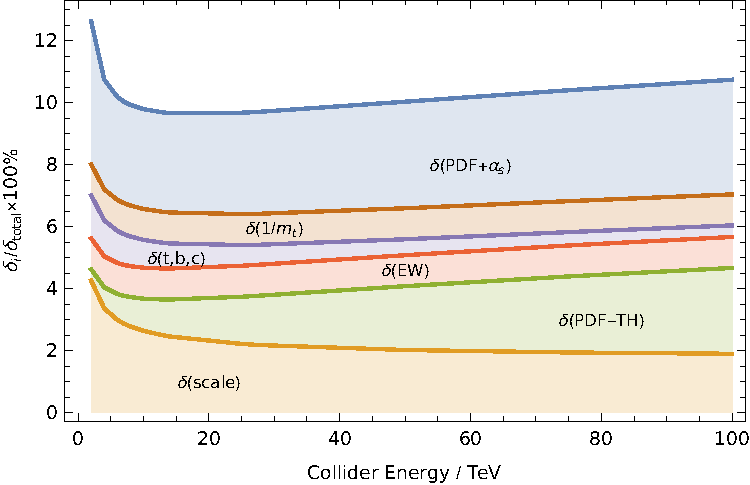
\includegraphics[width=0.8\textwidth]{figures/sources_of_unceratinty.pdf}
%         \caption*{Uncertainties for inclusive Higgs production \\
%         \color{gray}\small [HL-LHC: 1902.00134]}
%       \end{figure}
%     \end{column}
%   \end{columns}
% \end{frame}





% \section{N$^3$LO}

\begin{frame}{Theory requirements for PDFs at N3LO}
  \begin{itemize}
    \item Splitting functions for DGLAP evolution \\

    \item Variable flavor number scheme matching conditions \\
    $ f_i^{\left(n_f+1\right)}\left(x, Q^2\right)=A_{i j}\left(x, \alpha_s\right) f_j^{\left(n_f\right)}\left(x, Q^2\right) $
    \item DIS coefficient functions
    \item Hadronic cross sections,
  \end{itemize}

  Not all available at N3LO, what is the best we can do?
  \begin{itemize}
    \item Use N3LO calculations where known
    \item Construct approximate results where possible
    \item Account for theory uncertainties of the missing or incomplete higher order
  \end{itemize}

  Make optimal use of the existing information. More information can be included as it becomes available. No need to wait for complete N3LO results!
\end{frame}


\begin{frame}{Splitting functions}
  Complete results for the N3LO splitting functions are not yet available

  A lot of information exists (with important contributions from Liverpool and Edinburgh):
  \begin{itemize}
    \item large-$n_f$ limit
    \item small-$x$ limit
    \item large-$x$ limit
    \item Mellin Moments
  \end{itemize}
\end{frame}


\begin{frame}{Splitting functions}
  How can we use this information to construct approximate splitting functions?

  The approximation is performed in Mellin space as an expansion in $nf$, where any double counting terms present in the resummed small-$x$ and large-$x$ expressions are removed
  $\gamma_{i j}^{(3)}=\gamma_{i j, n_f}^{(3)}+\gamma_{i j, N \rightarrow \infty}^{(3)}+\gamma_{i j, N \rightarrow 0}^{(3)}+\gamma_{i j, N \rightarrow 1}^{(3)}+\widetilde{\gamma}_{i j}^{(3)}$.

  The remainder is constructed as a linear combination of interpolating functions:
  \begin{itemize}
    \item A function for the leading unknown large-N contribution
    \item A function for the leading unknown small-N contribution
    \item Functions for the subleading small-N and large-N contributions
  \end{itemize}

  Vary subleading contributions included in the basis of interpolating functions to estimate "incomplete higher order uncertainties" (IHOU) on the splitting functions. More details later
\end{frame}


\begin{frame}{Splitting functions}
  LO, NLO, NNLO and approximate N3LO splitting functions
  \begin{figure}
    \centering
    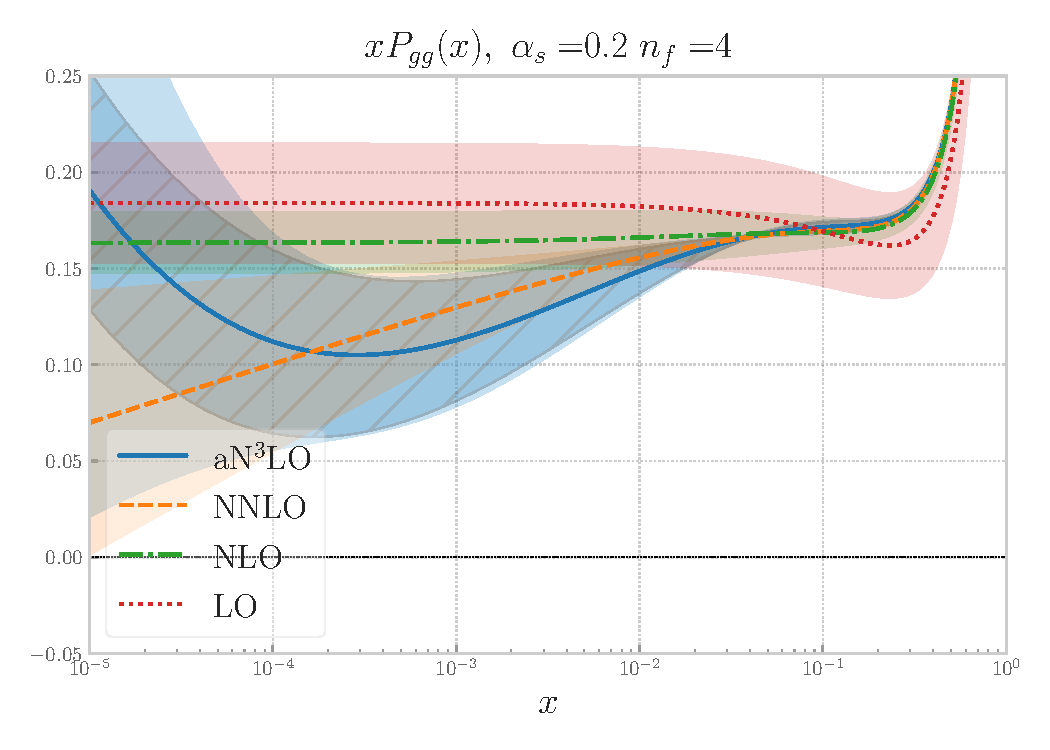
\includegraphics[width=.3\textwidth]{figures/gamma_gg_totu_logx.pdf}
    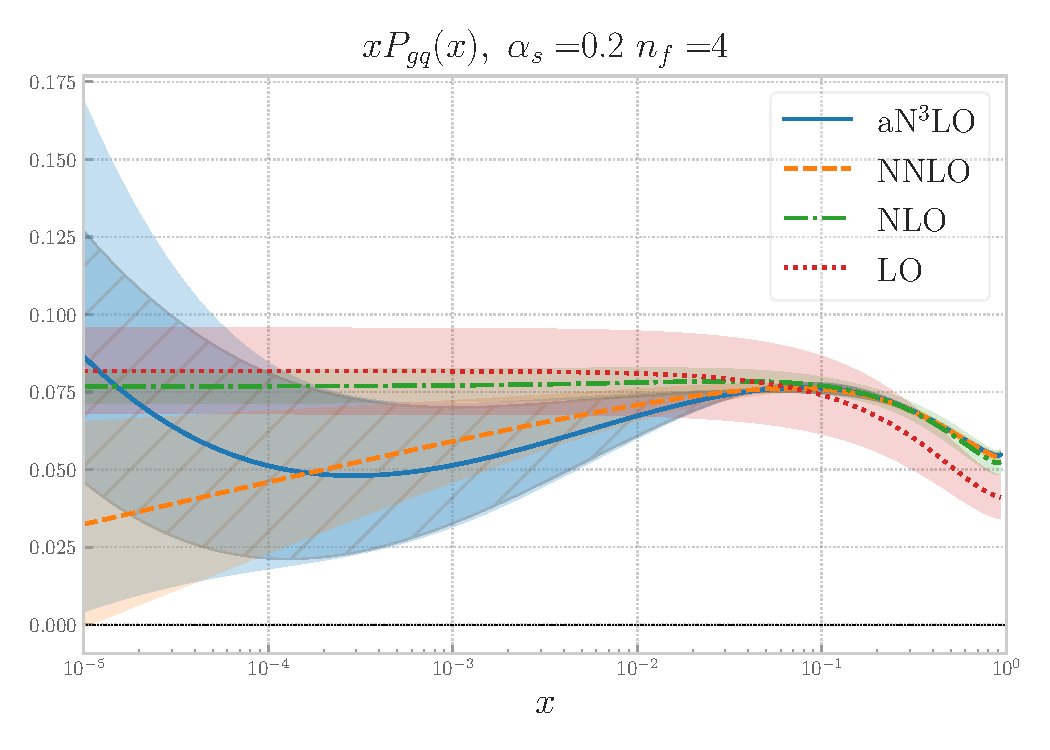
\includegraphics[width=.3\textwidth]{figures/gamma_gq_totu_logx.pdf} \\
    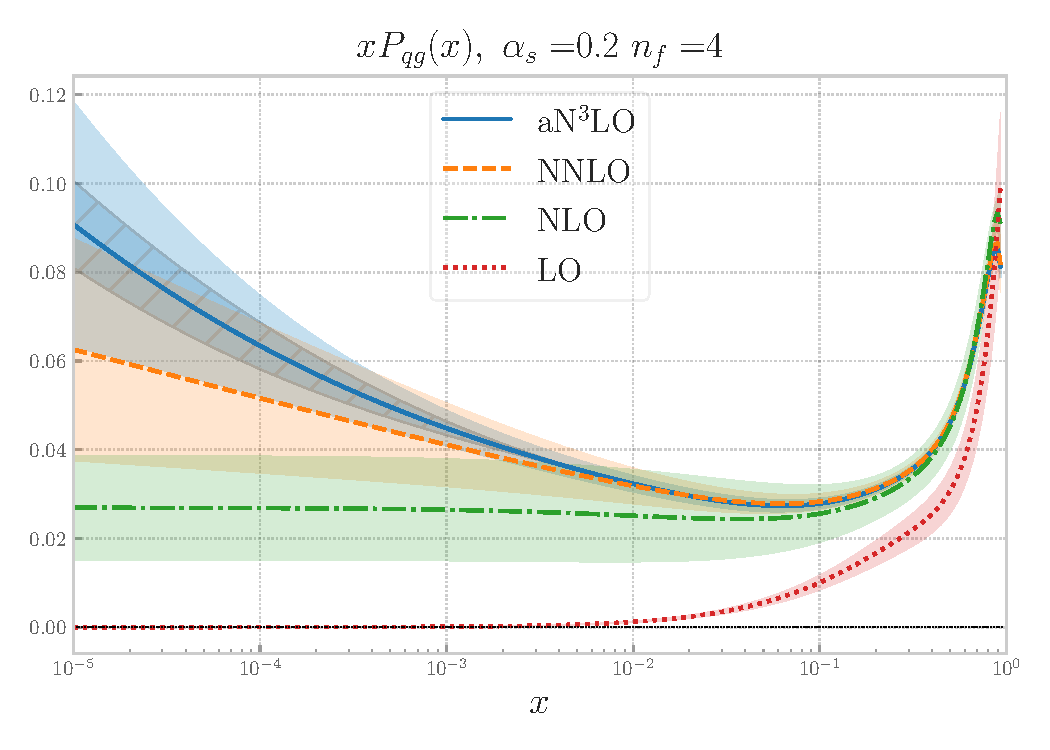
\includegraphics[width=.3\textwidth]{figures/gamma_qg_totu_logx.pdf}
    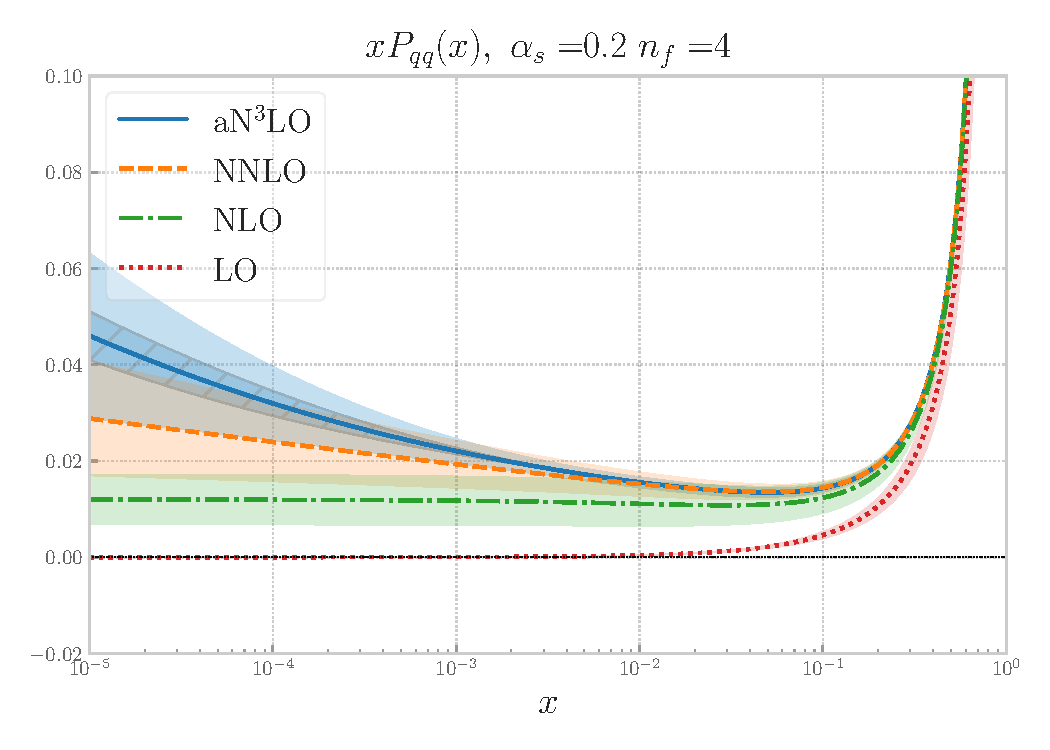
\includegraphics[width=.3\textwidth]{figures/gamma_qq_totu_logx.pdf}
  \end{figure}
  Shown uncertainties are estimated missing higher order uncertainty (MHOU) through factorization scale variations \\
  Light blue is sum in quadrature of MHOU and IHOU

  \begin{itemize}
    \item Good perturbative consistency within uncertainties
  \end{itemize}
\end{frame}



\begin{frame}{DGLAP evolution}
  NNPDF4.0 evolved from $Q=1.65$GeV to $Q=100$GeV
  \begin{figure}[!t]
    \centering
    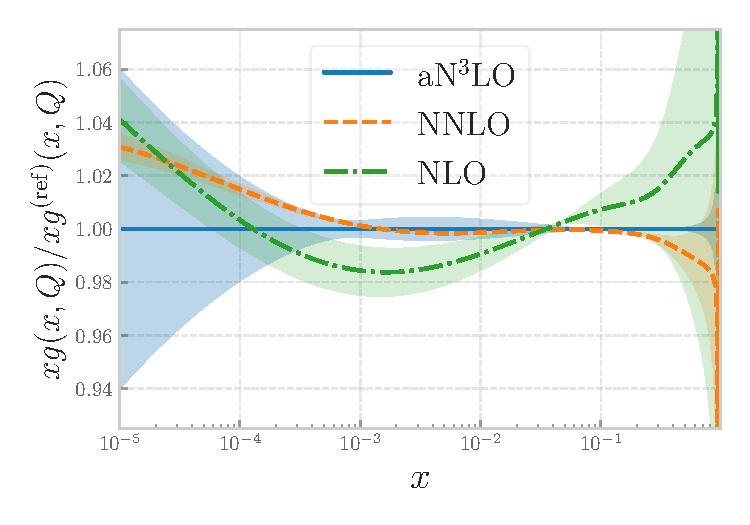
\includegraphics[width=0.3\textwidth]{figures/N3LOevolution-q100gev-ratios_expanded_0.pdf}
    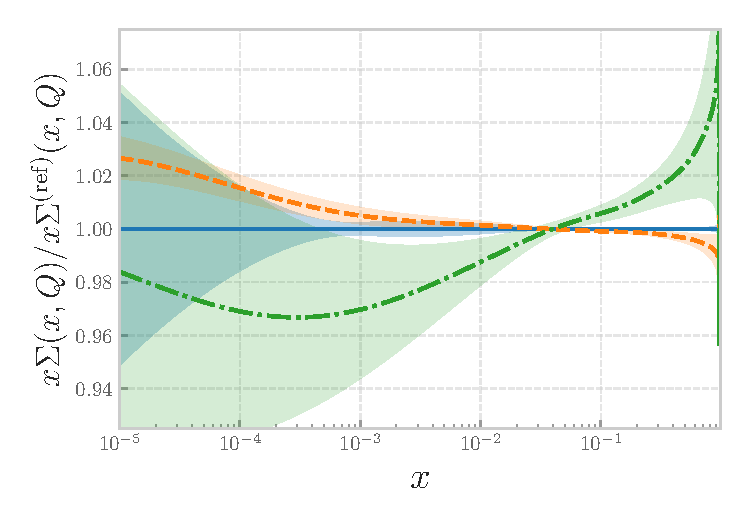
\includegraphics[width=0.3\textwidth]{figures/N3LOevolution-q100gev-ratios_expanded_1.pdf}\\
    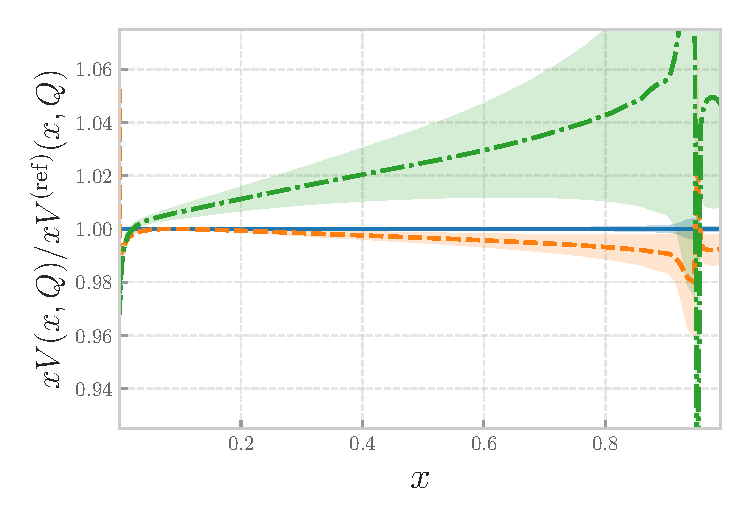
\includegraphics[width=0.3\textwidth]{figures/N3LOevolution-q100gev-ratios_expanded_2.pdf}
    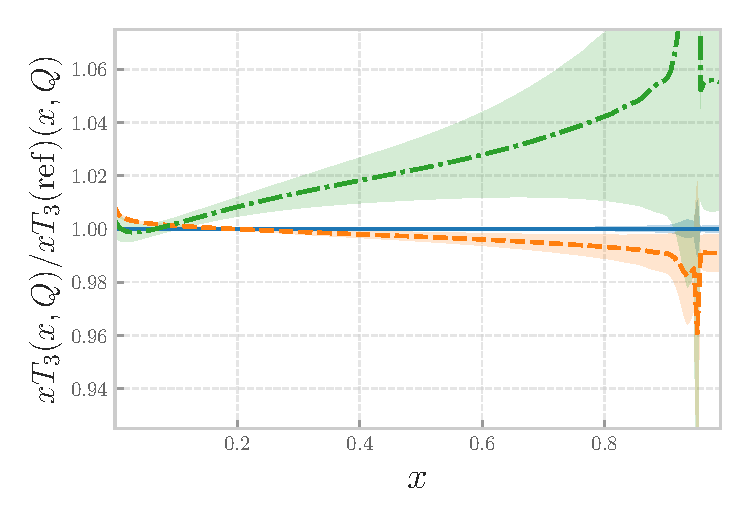
\includegraphics[width=0.3\textwidth]{figures/N3LOevolution-q100gev-ratios_expanded_3.pdf}
  \end{figure}
  \begin{itemize}
    \item Effects of N3LO corrections to DGLAP evolution at most percent level, except at small-$x$ and large-$x$
    \item Good perturbative convergence
  \end{itemize}
\end{frame}

\begin{frame}{DIS coefficient functions}
  \begin{itemize}
    \item DIS coefficient functions are known up to N3LO in the massless limit
    \item Massive coefficient functions can be constructed as a linear combination of the known limits
  \end{itemize}

  \begin{figure}[!t]
    \centering
    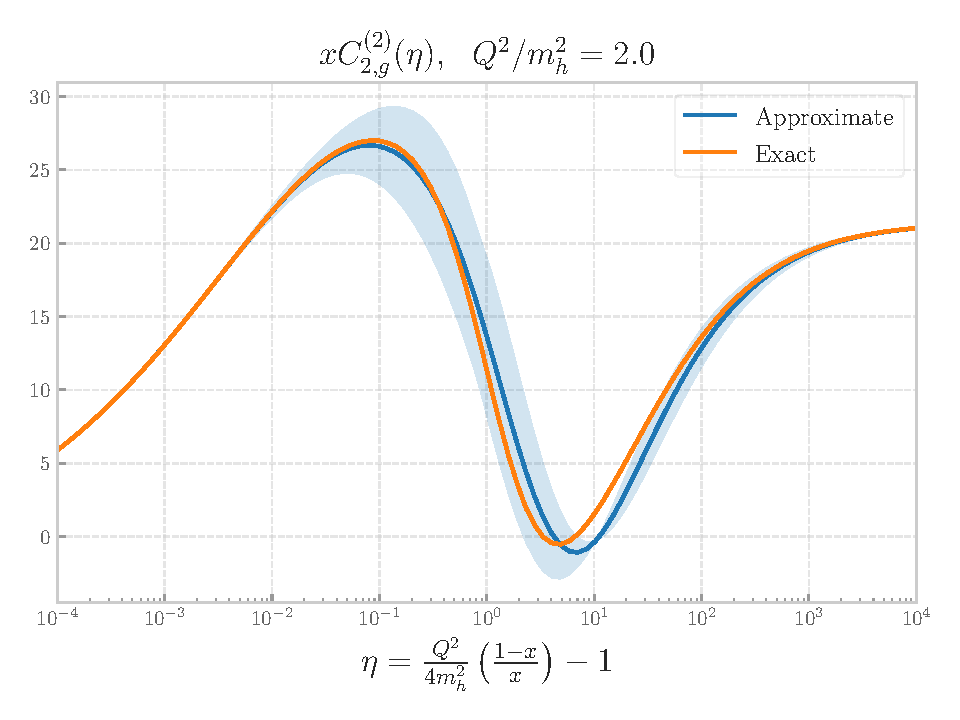
\includegraphics[width=.49\textwidth]{figures/C2g_2_Q2m2_2.0.pdf}
    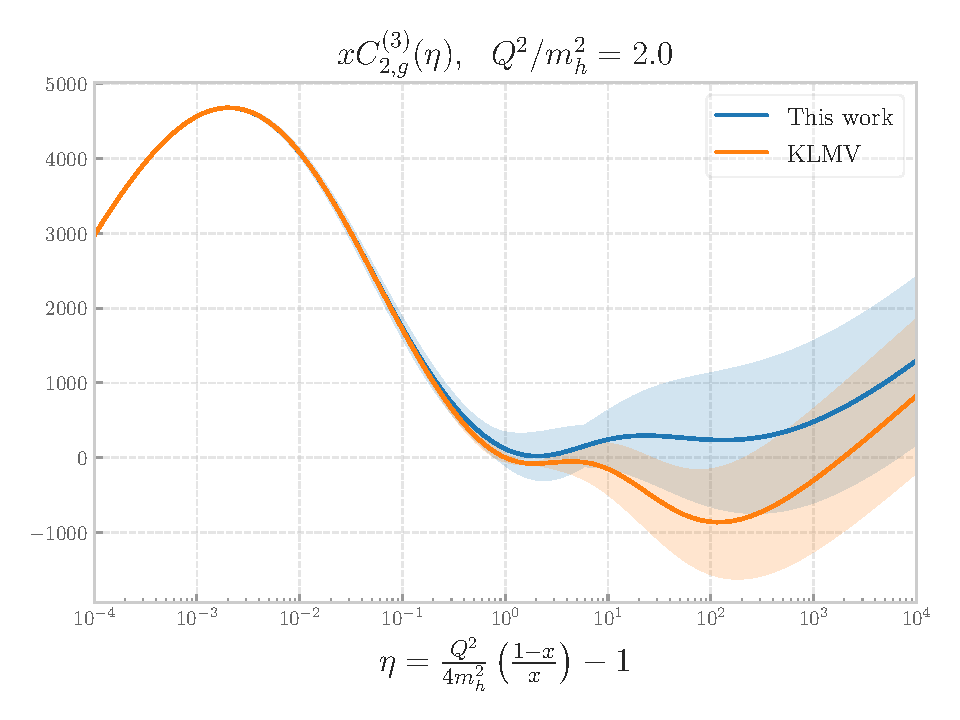
\includegraphics[width=.49\textwidth]{figures/C2g_3_Q2m2_2.0.pdf}
    NNLo and aN3LO
  \end{figure}
\end{frame}


\begin{frame}{DIS variable flavor number scheme}
  In a PDF fit different flavour number schemes are joined in a variable flavour number scheme (VFNS) to ensure reliable results from $Q^2\sim m_h^2$ up to $Q^2\gg m_h^2$

  The matching conditions encoding the transition between schemes have almost completely been computed up to N3LO

  The VFNS used in NNPDF is the FONLL scheme, constructed as
  $$F_\mathrm{FONLL}(Q^2,m_c)=F^{(n_f+1)}(Q^2,m_h=0)+F^{(n_f)}(Q^2,m_c)-\lim_{m_c\rightarrow 0}F^{(n_f)}(Q^2,m_h)$$

  Up to NNLO, FONLL was implemented expressing the terms in the r.h.s in terms of $\alpha_s$ and PDFs defined in the massless scheme

  FONLL is now implemented at ``observable level'' with simultaneous PDFs in different flavour number schemes, made possible thanks to the new \texttt{EKO} evolution code and \texttt{yadism} DIS library

  \begin{figure}[!t]
    \centering
    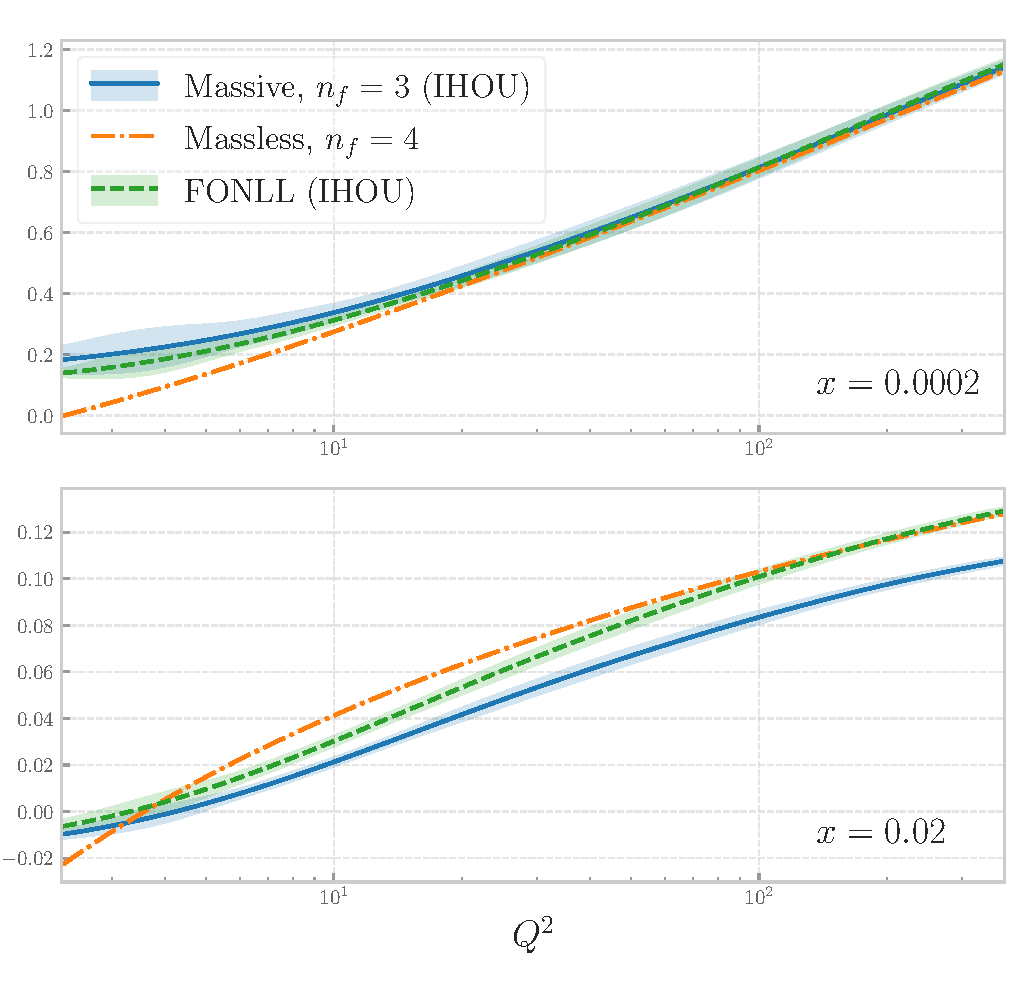
\includegraphics[width=0.3\textwidth]{figures/F2_charm_n3lo.pdf}
  \end{figure}

\end{frame}



\begin{frame}{DIS structure functions}
  \begin{figure}[!t]
    \centering
    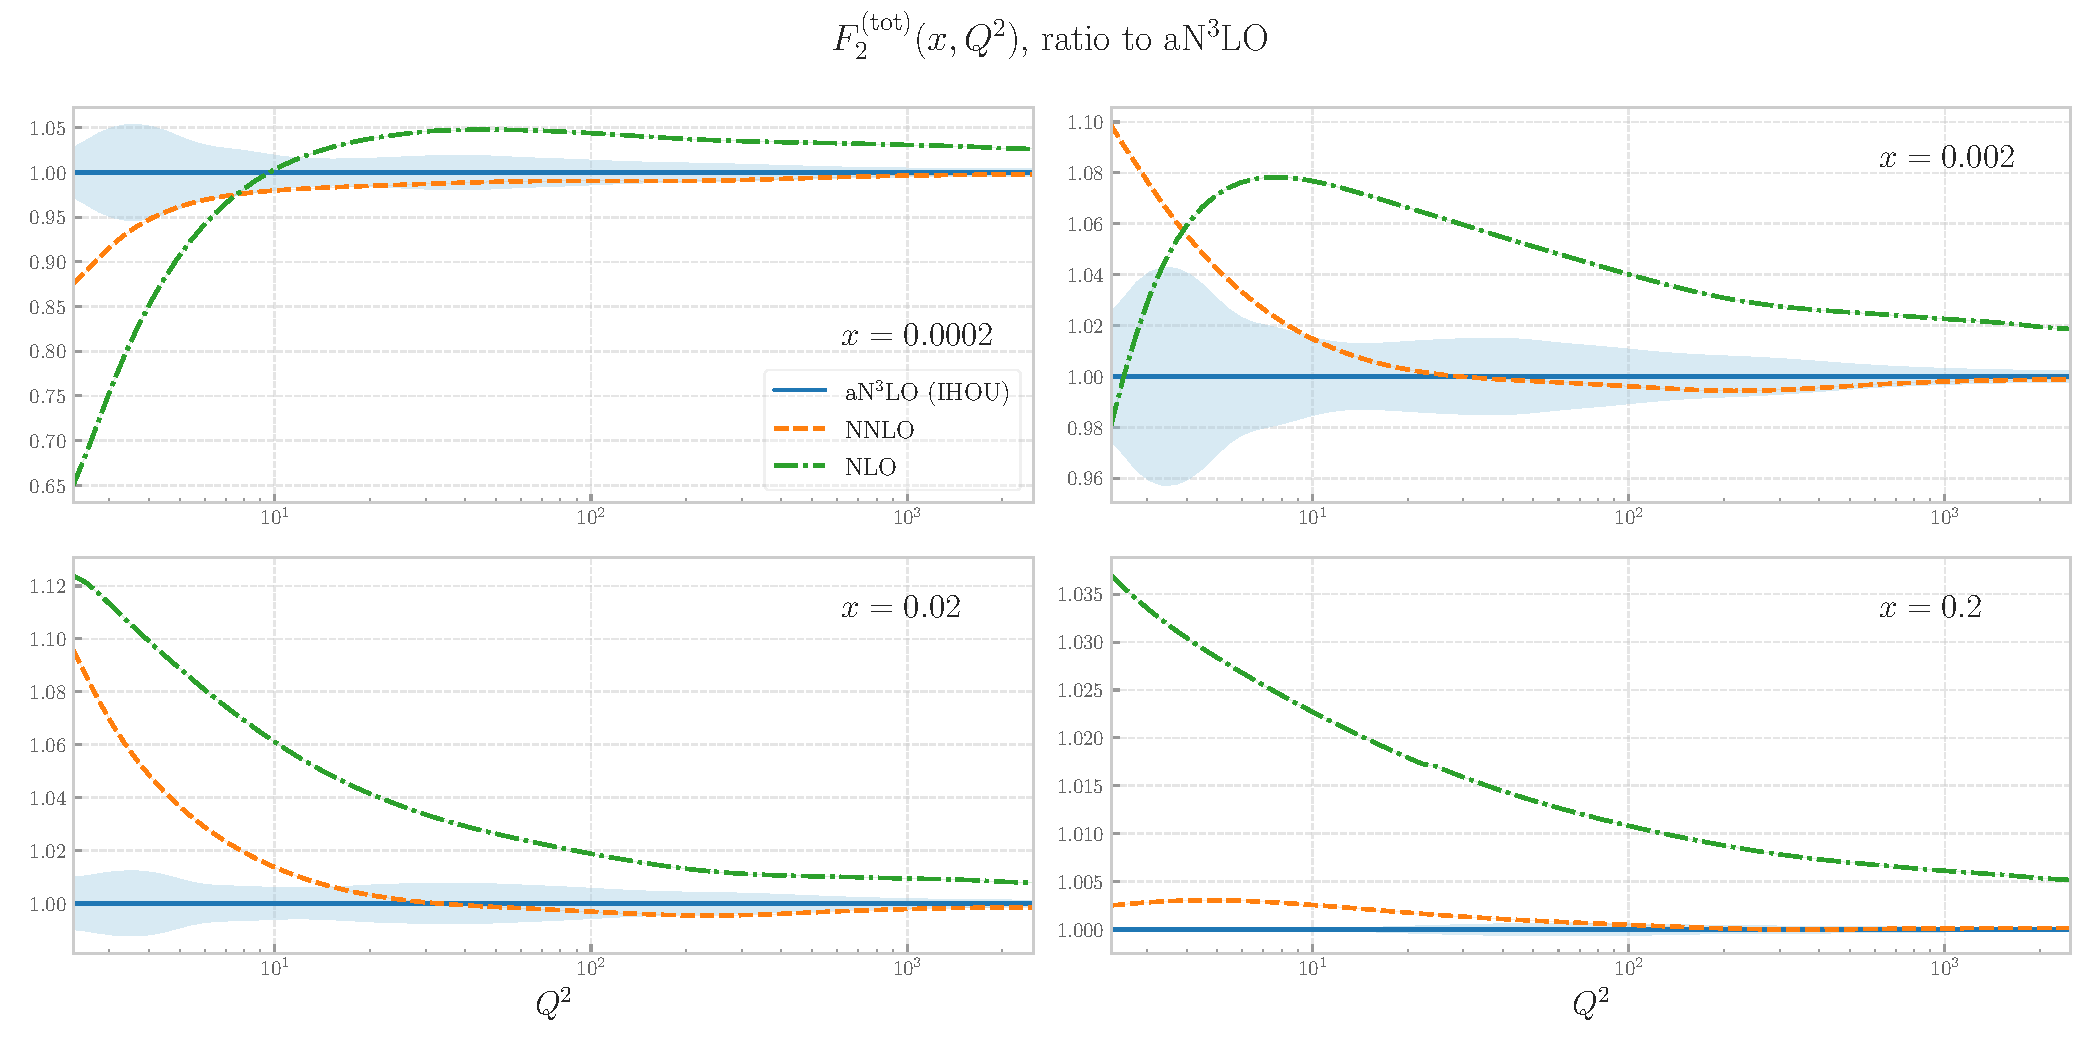
\includegraphics[width=0.8\textwidth]{figures/F2_total.pdf}
  \end{figure}
  \begin{itemize}
    \item unc is IHOU of the massive coefficient functions
    \item N3LO corrections are significant at low-$Q$
  \end{itemize}
\end{frame}


\begin{frame}{Hadronic processes}
  \begin{itemize}
    \item Corrections to collider DY and $W$ production can be included through k-factors
    \item N3LO effects around 1 to 2\%
    \item For many processes N3LO corrections are not available, for those we introduce MHOU
  \end{itemize}
  \begin{figure}[!t]
    \centering
    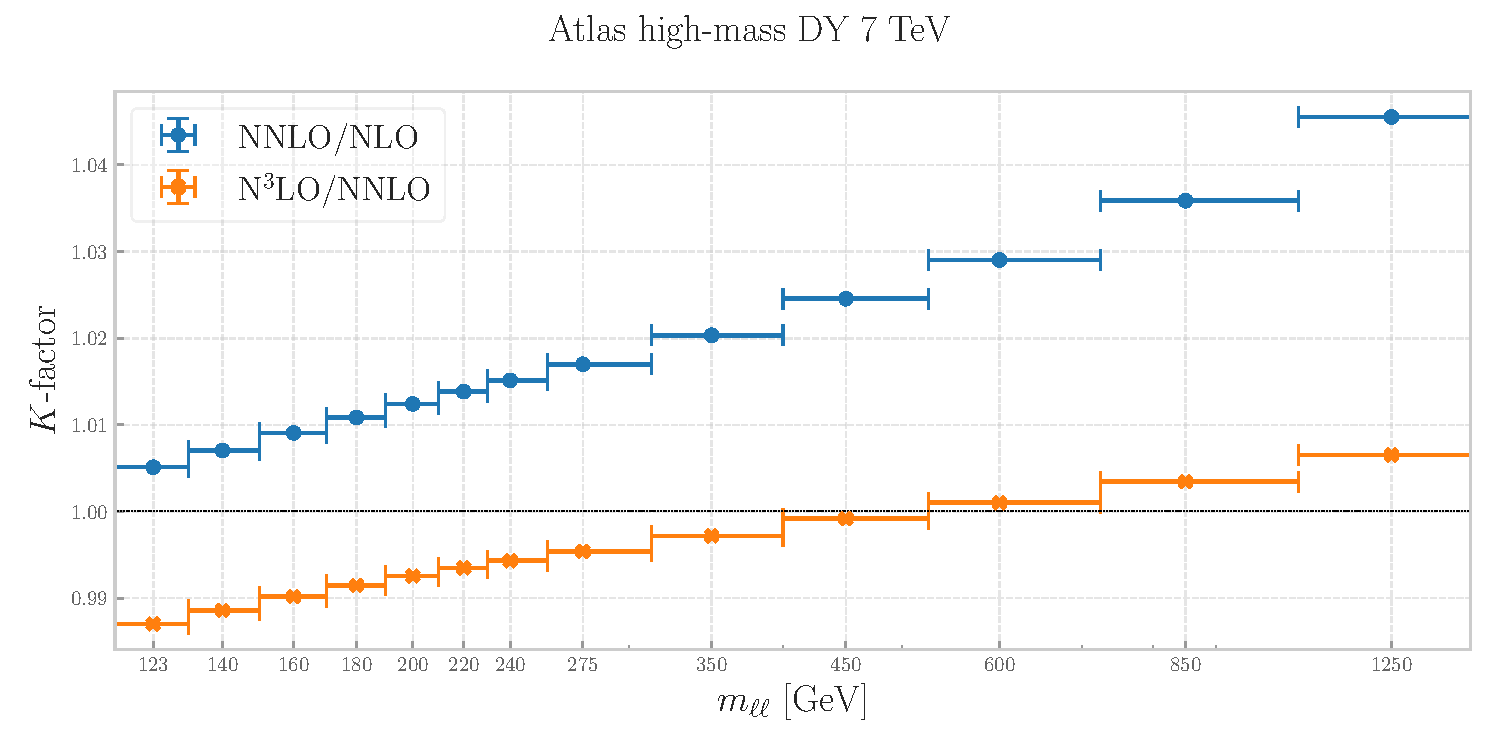
\includegraphics[width=.80\textwidth]{figures/kfactor_ATLASZHIGHMASS49FB.pdf}
  \end{figure}
\end{frame}


\section{MHOU}

\begin{frame}{Theory errors in a a PDF fit}
% include th covmat on same footing as exp covmat
% construct by varying fact and ren. scale var.
\end{frame}

\begin{frame}{Magnitude of theory uncertainties}
% show that for certain processes th unc is of same size as exp unc.
\end{frame}

\begin{frame}{Validate by comparing to known NNLO}
% show the validation plot
% we will see later the impact on the PDF/pheno
\end{frame}


\begin{frame}{Incomplete higher order uncertainties}
%
\end{frame}


\begin{frame}{NNPDF4.0 aN3LO}
% impact at PDF level of aN3LO and MHOU
\end{frame}

\begin{frame}{NNPDF4.0 aN3LO}
% impact at lumi level of aN3LO and MHOU
\end{frame}

\section{Phenomenology}

\begin{frame}{Higgs production}

\end{frame}


\begin{frame}{Drell-Yan}

\end{frame}


\begin{frame}{DIS at EIC}

\end{frame}


\section{Summary and outlook}
\begin{frame}{Incomplete higher order uncertainties}
  % outlook: combine N3LO+MHOU and QED
\end{frame}


\end{document}
